\documentclass[12pt]{article}
\usepackage[utf8]{inputenc}
\usepackage[a4paper, margin=2cm]{geometry}
\usepackage{multicol, caption}
\usepackage{authblk}
\usepackage[varg]{txfonts}
\usepackage{titlesec}
%\usepackage[T1]{fontenc}
%\usepackage{lmodern}
% \usepackage[english]{babel}


\usepackage{amsmath}
\usepackage{amssymb}
\usepackage{amsfonts}
\usepackage{graphicx}% Include figure files
\usepackage{dcolumn}% Align table columns on decimal point
\usepackage{bm}% bold math
\usepackage{hyperref}% add hypertext capabilities
\usepackage{minted}
\usepackage[autostyle]{csquotes}
\usepackage{wrapfig}

\usepackage[backend=biber,style=numeric]{biblatex}
\addbibresource{bib.bib}

\hyphenpenalty=10000
\exhyphenpenalty=10000

% CUSTOM FORMAT FOR SECTION
\titleformat{\section}[wrap]{\normalfont\bfseries}{\thesection.}{0.5em}{}
\titlespacing{\section}{12pc}{1.5ex plus .1ex minus .2ex}{1pc}
% CUSTOM SUBSECTION
\titleformat{\subsection}[wrap]{\normalfont\bfseries}{\thesubsection.}{0.5em}{}
\titlespacing{\subsection}{12pc}{1.5ex plus .1ex minus .2ex}{1pc}
% CUSTOM SUBSUBSECTION 
\titleformat{\subsubsection}[wrap]{\normalfont\bfseries}{\thesubsubsection.}{0.5em}{}
\titlespacing{\subsubsection}{12pc}{1.5ex plus .1ex minus .2ex}{1pc}

% CUSTOM LINE SPACING (Default 1.2 -> 1.2*1.25=1.5)
\linespread{1.25}

% CUSTOM NAMING
\renewcommand*\contentsname{Summary}

% CUSTOM FIGURES
\usepackage{import}
\usepackage{xifthen}
\usepackage{pdfpages}
\usepackage{transparent}
\newcommand{\incfig}[2][1]{
    \def\svgwidth{#1\textwidth}
    \input{#2.pdf_tex}
}

%CUSTOM APPENDIX
\usepackage[toc, page]{appendix}

\newenvironment{Figure}
  {\par\medskip\noindent\minipage{\linewidth}}
  {\endminipage\par\medskip}

\title{PHYS6006 Final Report \\
       Magnetospheric structure associated with high-latitude auroras}
\author[1]{J. Plank}
\author[2]{R. C. Fear}
\affil[1, 2]{Department of Physics and Astronomy, University of Southampton}
\date{April 2020}

\begin{document}\sloppy
% TITLE BLOCK
\maketitle

% ABSTRACT
\begin{abstract}
    \noindent\textit{Context:} Only case studies have been done on the magnetospheric structure associated with the formation of high latitude aurora, and the connection to interplanetary magnetic field direction is suspected but has never been quantified.\\
    \textit{Aims:} To produce a statistical survey on the relationship between a northward pointing interplanetary magnetic field and a phenomenon known as transpolar arcs.\\
    \textit{Methods:} Using data from the ESA satellite Cluster, and NASA's OMNI dataset, we analysed the average IMF $B_Z$ at high temperatures $T>20\ MK$ at increasing $Z$, covering the plasma sheet and the lobe. \\
    \textit{Results:} We found that there is no general correlation between high temperatures in the lobe and the presence of northward IMF, however there were several occasions when a connection was present (2002 and 2005), which could be explored further in a future report.
\end{abstract}

\pagebreak

\tableofcontents
\addtocontents{toc}{~\hfill\textbf{Page}\par}

\pagebreak

% % SWITCH TO 2 COLUMNS
% \begin{multicols}{2}

\section{INTRODUCTION}
Earth and the Sun are connected by more than just gravity, magnetic interactions between the two bodies are the cause of some of the most dramatic and complex phenomena on Earth. The most well known of these is the aurora (Borealis in the northern hemisphere and Australis in the southern). More commonly known as the northern and southern lights, these light shows come as a result of charged particles flowing along the Sun's magnetic field lines (known as solar wind) and making their way down to Earth to form the auroral oval \cite{AAAspaceweather}. The Sun's violent nature is also transmitted to Earth via its magnetic field, known as the `Interplanetary magnetic field` (IMF). This can result in satellite damage, radiation hazards to astronauts and airline passengers, telecommunications problems, and outages of power and electronics systems \cite{AAAspaceweather}.

The modern theory for the formation of aurora was first proposed by Kristian Birkeland in 1903 \cite{birkeland2018norwegian}. He said that auroras are produced when solar wind encounters the geomagnetic field. The result of this is the formation of the plasmasphere in the equatorial plane of Earth's magnetic field \cite{cosmicelectrodyn}.

%ADD MORE ABOUT BACKGROUND TO THIS PROJECT AND AIMS
One type of aurora that occurs at high latitudes on Earth is the transpolar arc. So far, only case studies have been done on how changes in the magnetic field far from Earth are associated with these auroras. In this project, we aim to complete a broader statistical survey that will help to determine how high-temperatures in the magnetosphere lobes are related to times when the magnetic field from the Sun points northward once it has travelled to Earth. This could lead to a better understanding of why these changes in Earth's magnetic field have taken place. We will also begin a comparison of the times that high temperatures are spotted by ESA's Cluster satellites and the times when transpolar arcs are spotted.

\section{THEORETICAL BACKGROUND}
\hfill \\
\hfill

\subsection{Structure of Earth's magnetic field}
Figure \ref{fig:plasmasphere} is a representation of the solar-terrestrial environment. Solar wind, travelling with the interplanetary magnetic field from the sun \cite{Svalgaard_2010}, is coming from the left. It collides with the terrestrial magnetic field at supersonic speeds, creating a bow shock wave in front of the magnetosphere - the region where magnetic field lines connect to Earth at both ends - the boundary of the magnetosphere is the magnetopause. Supersonic solar winds compress at this boundary creating a magnetosheath between the magnetopause and the bow shock \cite{BSPP}.

\begin{Figure}
    \begin{minipage}[c]{0.57\textwidth}
        \centering
        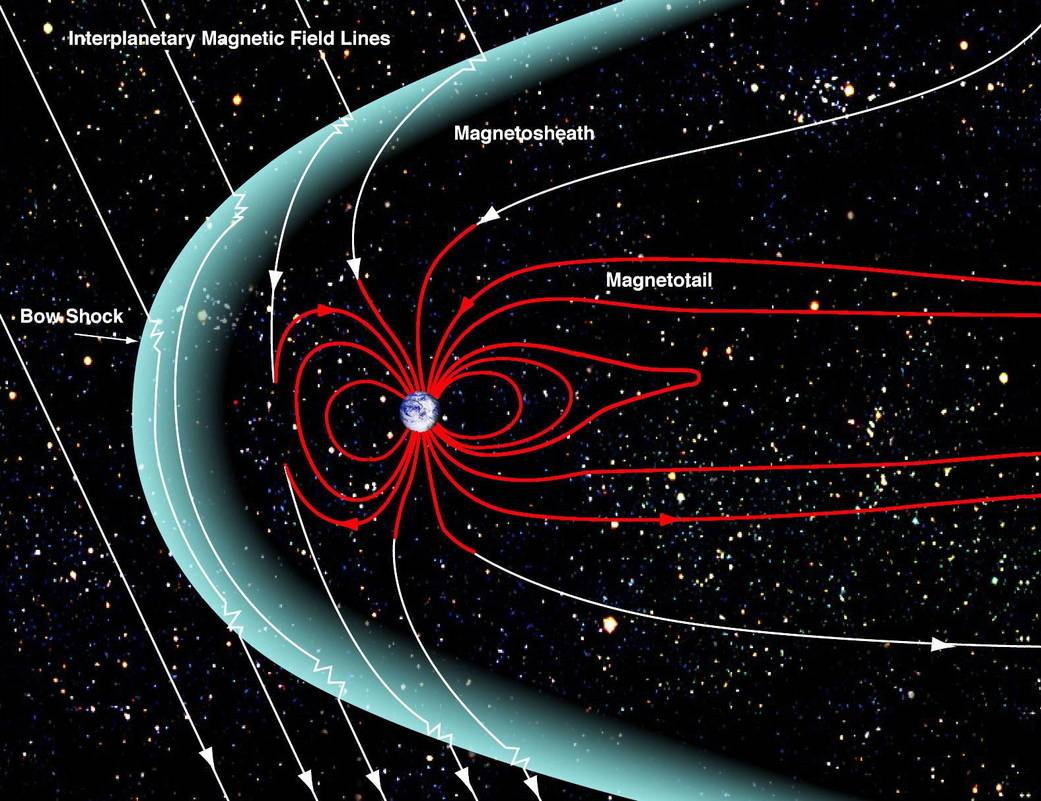
\includegraphics[width=0.7\textwidth]{NASA-Magnetosphere.jpeg}
    \end{minipage}\hfill
    \begin{minipage}[c]{0.4\textwidth}
        \captionof{figure}{Representation of the solar-terrestrial magnetic interaction. The sun is located to the left, producing solar winds and the IMF. Solar winds collide with the terrestrial magnetic field at supersonic speeds, creating a bow shock wave which encases the magnetosphere in a magnetosheath of compressed solar wind \cite{BSPP}. (Image courtesy of NASA)}
        \label{fig:plasmasphere}
    \end{minipage}
\end{Figure}

\subsection{Coordinate Systems}
Geocentric Solar Ecliptic (GSE) and Geocentric Solar Magnetic (GSM) are two similar coordinate systems used when studying the magnetosphere. Both have the Earth as the origin, and $+X$ pointing towards the sun. In GSE, $+Z$ is pointed perpendicularly upwards from the plane of Earth's orbit around the Sun. In GSM, $Z$ is the projection of Earth's magnetic dipole axis onto the plane perpendicular to $X$, with positive pointing north.

\begin{Figure}
    \begin{minipage}[c]{0.48\textwidth}
        \centering
        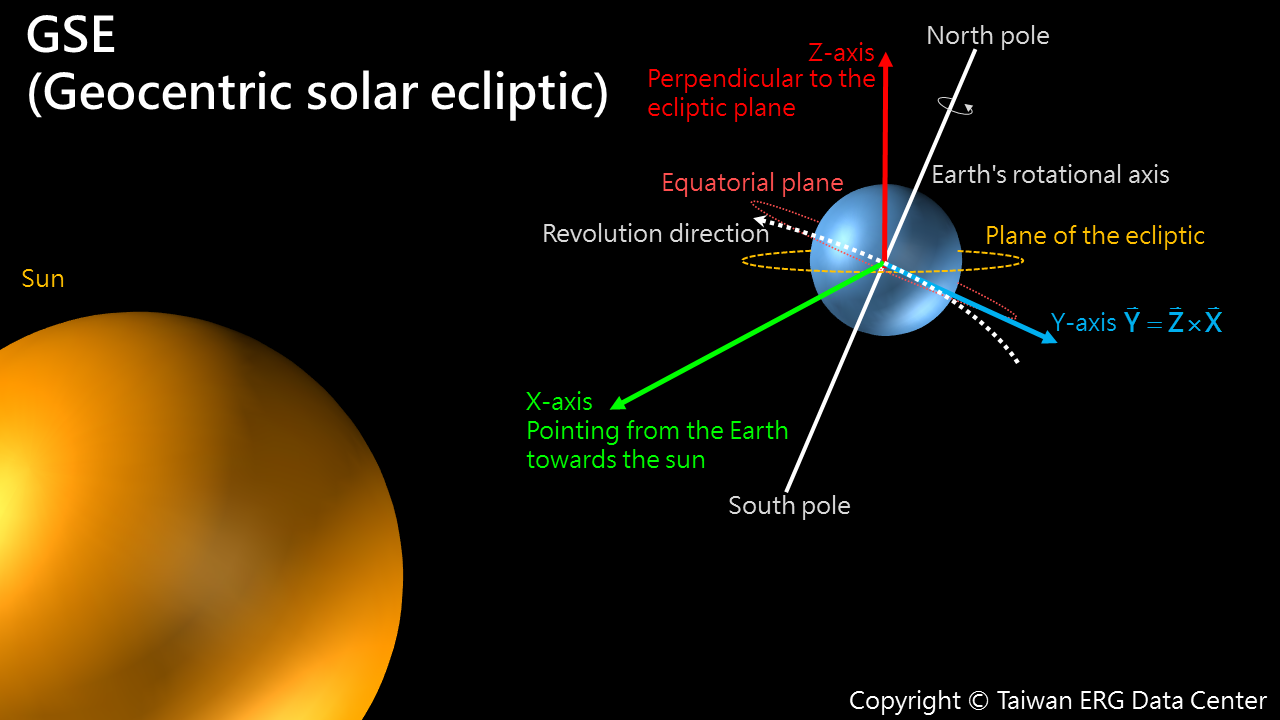
\includegraphics[width=\textwidth]{GSE.png}
    \end{minipage}
    \begin{minipage}[c]{0.48\textwidth}
        \centering
        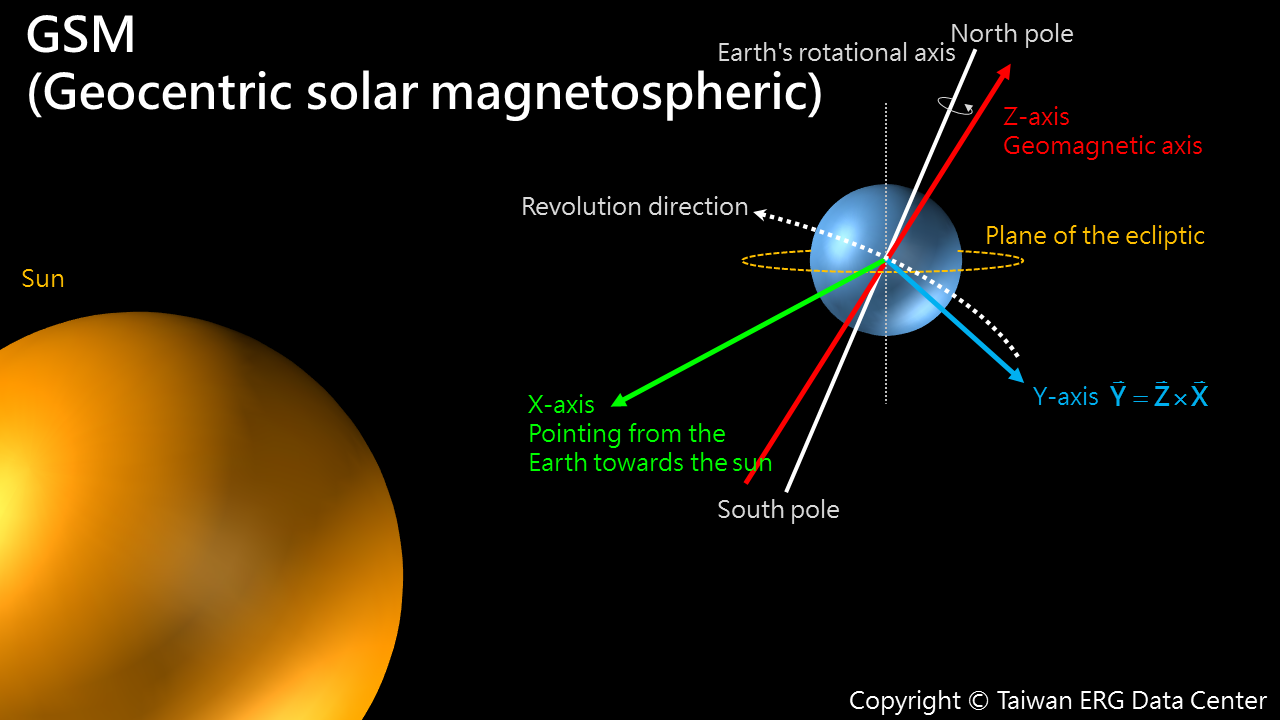
\includegraphics[width=\textwidth]{GSM.png}
    \end{minipage}
    \captionof{figure}{The GSE (left) and GSM (right) coordinate systems. Image credit: \cite{taiwanergdatacenter}.}
\end{Figure}

\subsection{The Interplanetary Magnetic Field}
Magnetic field lines are said to be ``frozen in`` to the solar wind plasma, the IMF is carried into the interplanetary region of space by solar wind from the sun. The mechanism for this is known as Alfvén's theorem, first proposed in 1942 \cite{alfven_1942}. 

Frozen-in flux/flow occurs when the magnetic Reynolds number is much greater than 1.

%Maybe put in an appendix?

Magnetohydrodynamic induction equation (Appendix \ref{app:mhd}):
\begin{align}
    \frac{\partial \textbf{B}}{\partial t} &= \nabla \times (\textbf{V}\times\textbf{B})+\frac{1}{\mu_0\sigma}\nabla^2\textbf{B}
\end{align}

Where the first term is the convective term and the second is diffusive. $\textbf{B}$ is the magnetic field, \textbf{V} is the velocity vector, $\mu_0$ is the permeability of free space and $\sigma$ is conductivity. The magnetic Reynolds number $R_m$ is defined as:
\begin{align}
    R_m&=\frac{\text{Convective term}}{\text{Diffusive term}} \nonumber\\
    &=\frac{|\nabla\times(\textbf{V}\times\textbf{B})|}{|\nabla^2\textbf{B}/\mu_0\sigma|}
\end{align}

Therefore if $R_m>1$ then the convective term dominates and if $R_m<1$ the diffusive term dominates. In the convective limit (when $R_m>>1$) then:
\begin{equation}
    \frac{\partial\textbf{B}}{\partial t}=\nabla\times(\textbf{V}\times\textbf{B})
    \label{eq:convLim}
\end{equation}

Faraday's law states that $\partial\textbf{B}/\partial t=-\nabla\times\textbf{E}$, so in the convective limit:
\begin{equation}
    \textbf{E}=-\textbf{V}\times\textbf{B}
\end{equation}

\begin{wrapfigure}{r}{0.4\textwidth}
    \hspace{1.5cm}
    \vspace{-5mm}
    \incfig[0.38]{frozen-in}
    \vspace{5mm}
\end{wrapfigure}

Consider a surface $S$ (see diagram), the magnetic flux passing through that surface is $\Phi=\int_S\textbf{B}.d\textbf{S}$. The change in magnetic flux through the surface can then be written as:

\begin{equation}
    \frac{d\Phi}{dt} = \int_s\frac{\partial\textbf{B}}{\partial t}.d\textbf{S} + \frac{d\Phi_C}{dt}
\end{equation}

Where $d\Phi_C/dt$ is due to the plasma motion causing a change in the surface.
This change (red box in diagram) has area $\textbf{V}dt\times d\textbf{l}$. The flux through this area is $\textbf{B}.(\textbf{V}dt\times d\textbf{l})$. Therefore:

\begin{align}
    \frac{d\Phi_C}{dt}&=\int_l\textbf{B}.(\textbf{V}\times d\textbf{l}) \nonumber\\
    &=-\int_S\nabla\times(\textbf{V}\times\textbf{B}).d\textbf{S}
\end{align}
from Stokes' theorem.

So the rate of change of flux through the surface is:
\begin{align}
    \frac{d\Phi}{dt}&=\int_S\frac{\partial\textbf{B}}{\partial t}.d\textbf{S}-\int_S\nabla\times(\textbf{V}\times\textbf{B}).d\textbf{S} \nonumber\\
    &= \int_S\left[\frac{\partial\textbf{B}}{\partial t}-\nabla\times(\textbf{V}\times\textbf{B})\right].d\textbf{S} \nonumber\\
    &= 0\text{ (eq \ref{eq:convLim})}
\end{align}

So, for $R_m >> 1$ the rate of change of the flux through a surface is 0. This means that the plasma must move with the field - or that the field must move with the plasma. Consider the thermal and magnetic energy densities ($W_T$ and $W_B$) to determine which dominates:

\begin{equation}
    \beta=\frac{W_T}{W_B}
\end{equation}

Where $\beta$ is the plasma beta. If $\beta>>1$ then the particle energy is dominant and it is the particle motion that carries the magnetic field. When $\beta<<1$ magnetic energy dominates and the plasma is frozen to magnetic field lines.

\subsubsection{Parker spiral}

Because of the rotation of the sun, solar wind (along with IMF) follows a spiral pattern similar to that produced by droplets of water as a wet tennis ball is thrown into the air with rapid spin. These field lines are `open`, i.e. they have an origin, but instead of returning to a corresponding region at the opposite pole, extend indefinitely into space \cite{imfUptoLat16}. 

At the Sun's magnetic equator, field lines originating from the northern and southern hemispheres run parallel to each other but are oppositely directed - creating a thin current sheet known as the ``Heliospheric current sheet``. This sheet is twisted and warped due to the difference in rotational and magnetic axes and a quadrupole moment in the sun's magnetic field - it also has a spiral shape of the same form as described above \cite{alfven_1942, ParkerSpiral}.

Since the orbital plane of the Earth is located almost along the rotation axis of the sun, we experience regular shifts in direction of flow of the IMF because the heliospheric current sheet is sometimes above and sometimes below the planet. 

When the IMF has a southward component, the northward pointing terrestrial field lines are allowed to merge in a process known as reconnection. However, when the IMF is northward, the structure of the magnetosphere is not well understood \cite{Fear1506}.

\subsection{Reconnection and Aurora}
The auroral lights, pictured in Fig.\ref{fig:auroraPic}, are a result of charged particles from the sun being accelerated towards the ionosphere - Earth's upper atmosphere - where they collide with gas molecules, each molecule causing a different colour to be emitted. 
E.g. Green (the most common colour) is caused by collisions with atomic oxygen ($557.7 nm$) \cite{hollier, BSPP}. Intense aurora will have an emission rate of several million Rayleigh ($1R=10^6 photons/cm^2s$) and most often appear as east-west aligned bands known as auroral arcs \cite{BSPP}.

\begin{Figure}
    \begin{minipage}[c]{0.67\textwidth}
        \centering
        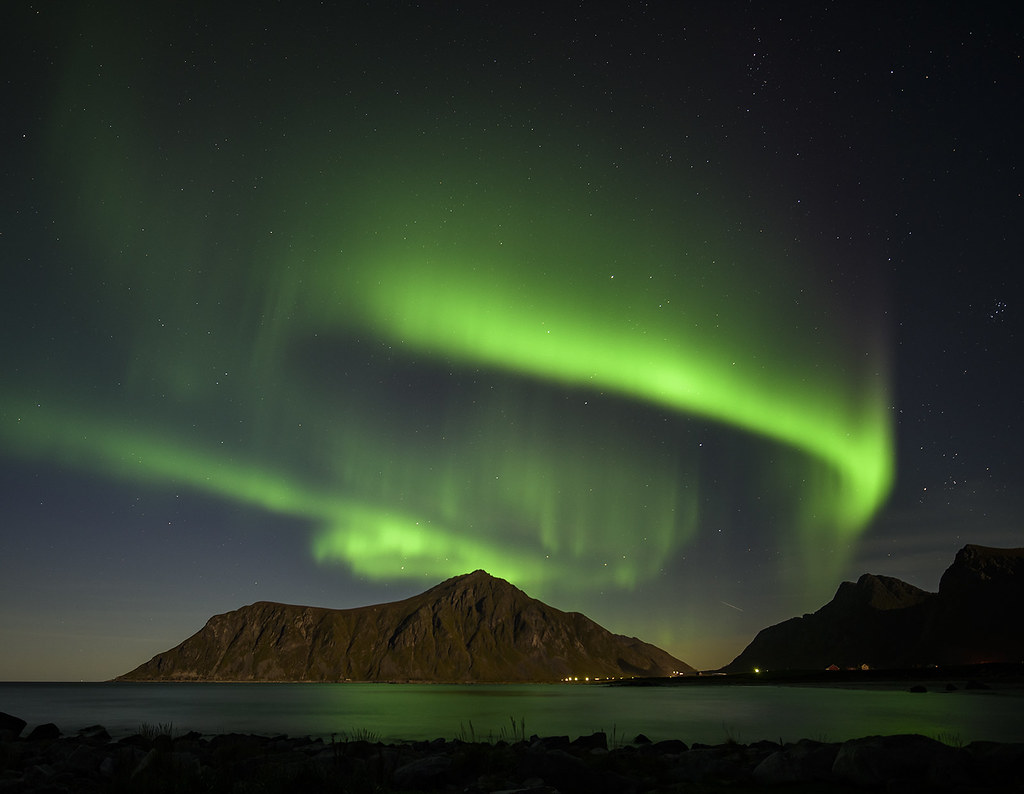
\includegraphics[width=0.8\linewidth]{nothernLights.jpg}
    \end{minipage}
    \begin{minipage}[c]{0.3\textwidth}
        \captionof{figure}{The Aurora Borealis, photographed in 2015 \cite{torino071_2015}.}
        \label{fig:auroraPic}
    \end{minipage}
\end{Figure}

Reconnection is a process that allows magnetic fields from separate domains to become joined to one another. When IMF is southward, reconnection occurs in a smooth cycle known as the Dungey cycle \cite{dungeyCycle} which is explained in Fig.\ref{fig:dungey}. Aurora is observed at latitudes of approximately $70^{\circ}$ because that is the boundary between the closed lines and the open ones at the polar cap (lobe).

%EXPLANATION OF RECONNECTION HERE

\begin{Figure}
    \centering
    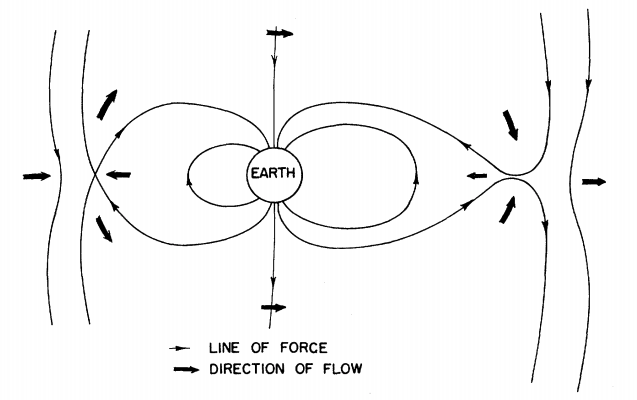
\includegraphics[width=0.6\linewidth]{dungeyCycle.png}
    \captionof{figure}{Sketch of the Dungey cycle. IMF is assumed to be coming from the left. On the right hand side of the diagram, magnetotail reconnection is happening. Open field lines are being compressed together, eventually joining to form a closed field line that `snaps back` towards Earth, the reconnection happens typically at a radius of $\approx100R_e$. Heating and acceleration of the plasma occurs as the newly created closed field line rapidly shortens in length. The magnetic flux will then flow around to the dayside of the planet (LHS of the sketch) where it gets pushed up against the solar wind. Once again, this pressure eventually reaches a point where the field lines of the IMF and the terrestrial field merge, creating an open line with its foot on the polar cap. This line gets pushed back over to the night-side of the planet where magnetotail reconnection can happen once again (Sketch from \cite{dungeyCycle}).}
    \label{fig:dungey}
\end{Figure}

Aurora at very high latitudes are rare, but can occur in an event known as a transpolar arc \cite{polarAurora1, polarAurora2} (see figure \ref{fig:TPA}). There is much debate on their formation, one theory was proposed by Milan \textit{et al} in \cite{TPAdebate}, where flux in the magnetotail lobes - the open field line region that maps down to the polar cap - reconnects but is trapped in the magnetotail. Transpolar arcs occur when the IMF is northward, which would explain why flux gets trapped in the magnetotail, there is a blockage created because dayside reconnection cannot occur.

\begin{Figure}
    \begin{minipage}[c]{0.4\textwidth}
        \centering
        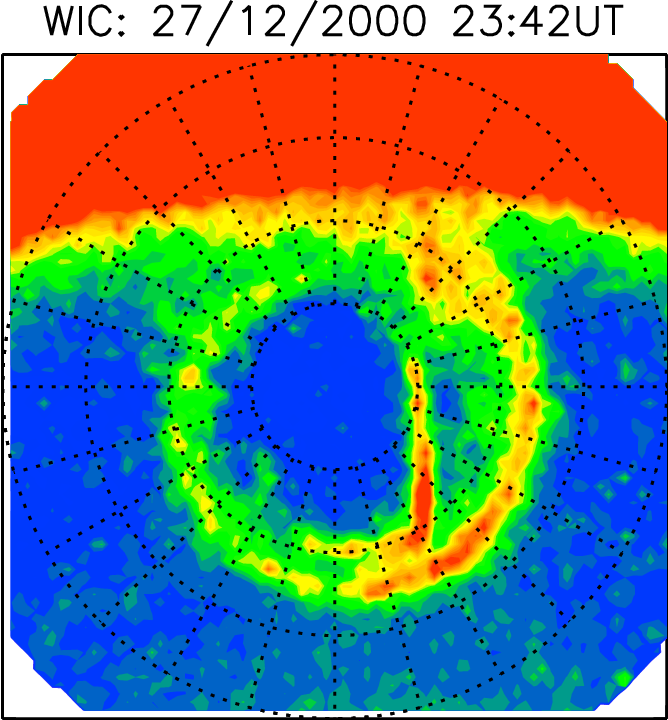
\includegraphics[width=0.9\textwidth]{transpolar_arc.png}
    \end{minipage}
    \begin{minipage}[c]{0.57\textwidth}
        \captionof{figure}{An example of a transpolar arc observed by Fear and Milan \cite{Fear2012TheID}. Dayglow is visible at the top of the image, the auroral oval is also visible as a circle in the centre of the image. The transpolar arc is the thin red band that stretches from the night side of the planet (bottom) into the polar cap region. An observer standing underneath a transpolar arc and looking up would see something that looks just like the normal aurora. The only significant difference is they are standing at a latitude that under normal circumstances would be far too high to see any aurora.}
        \label{fig:TPA}
    \end{minipage}
\end{Figure}

\section{OBSERVATIONS}
The majority of observations in this report come from Cluster, a group of four satellites built by ESA and launched in pairs on Soyuz rockets from Baikonur on the 16th July and 9th August 2000. They fly in a 57hr elliptical polar orbit and are arranged in a tetrahedral formation with a separation of between a few hundred and a few thousand km.

\subsection{Limitations of Cluster's orbit}
The orbit of cluster varies throughout the year. For significant portions of the year the satellite is well outside of the lobes, therefore the best months to extract data are July-October every year, where the spacecraft spends the majority of its time in the tail, and does not enter the magnetosheath. 

Figure \ref{fig:ClusterPos} shows Cluster's orbit through the month of September 2005 as an example, it does not cross the predicted magnetopause boundary (outer dotted parabola). Cluster will also cross through the plasmasphere in every orbit. This leaves the grey shaded region as the area of interest.

\begin{Figure}
    \begin{minipage}[c]{0.4\textwidth}
        \centering
        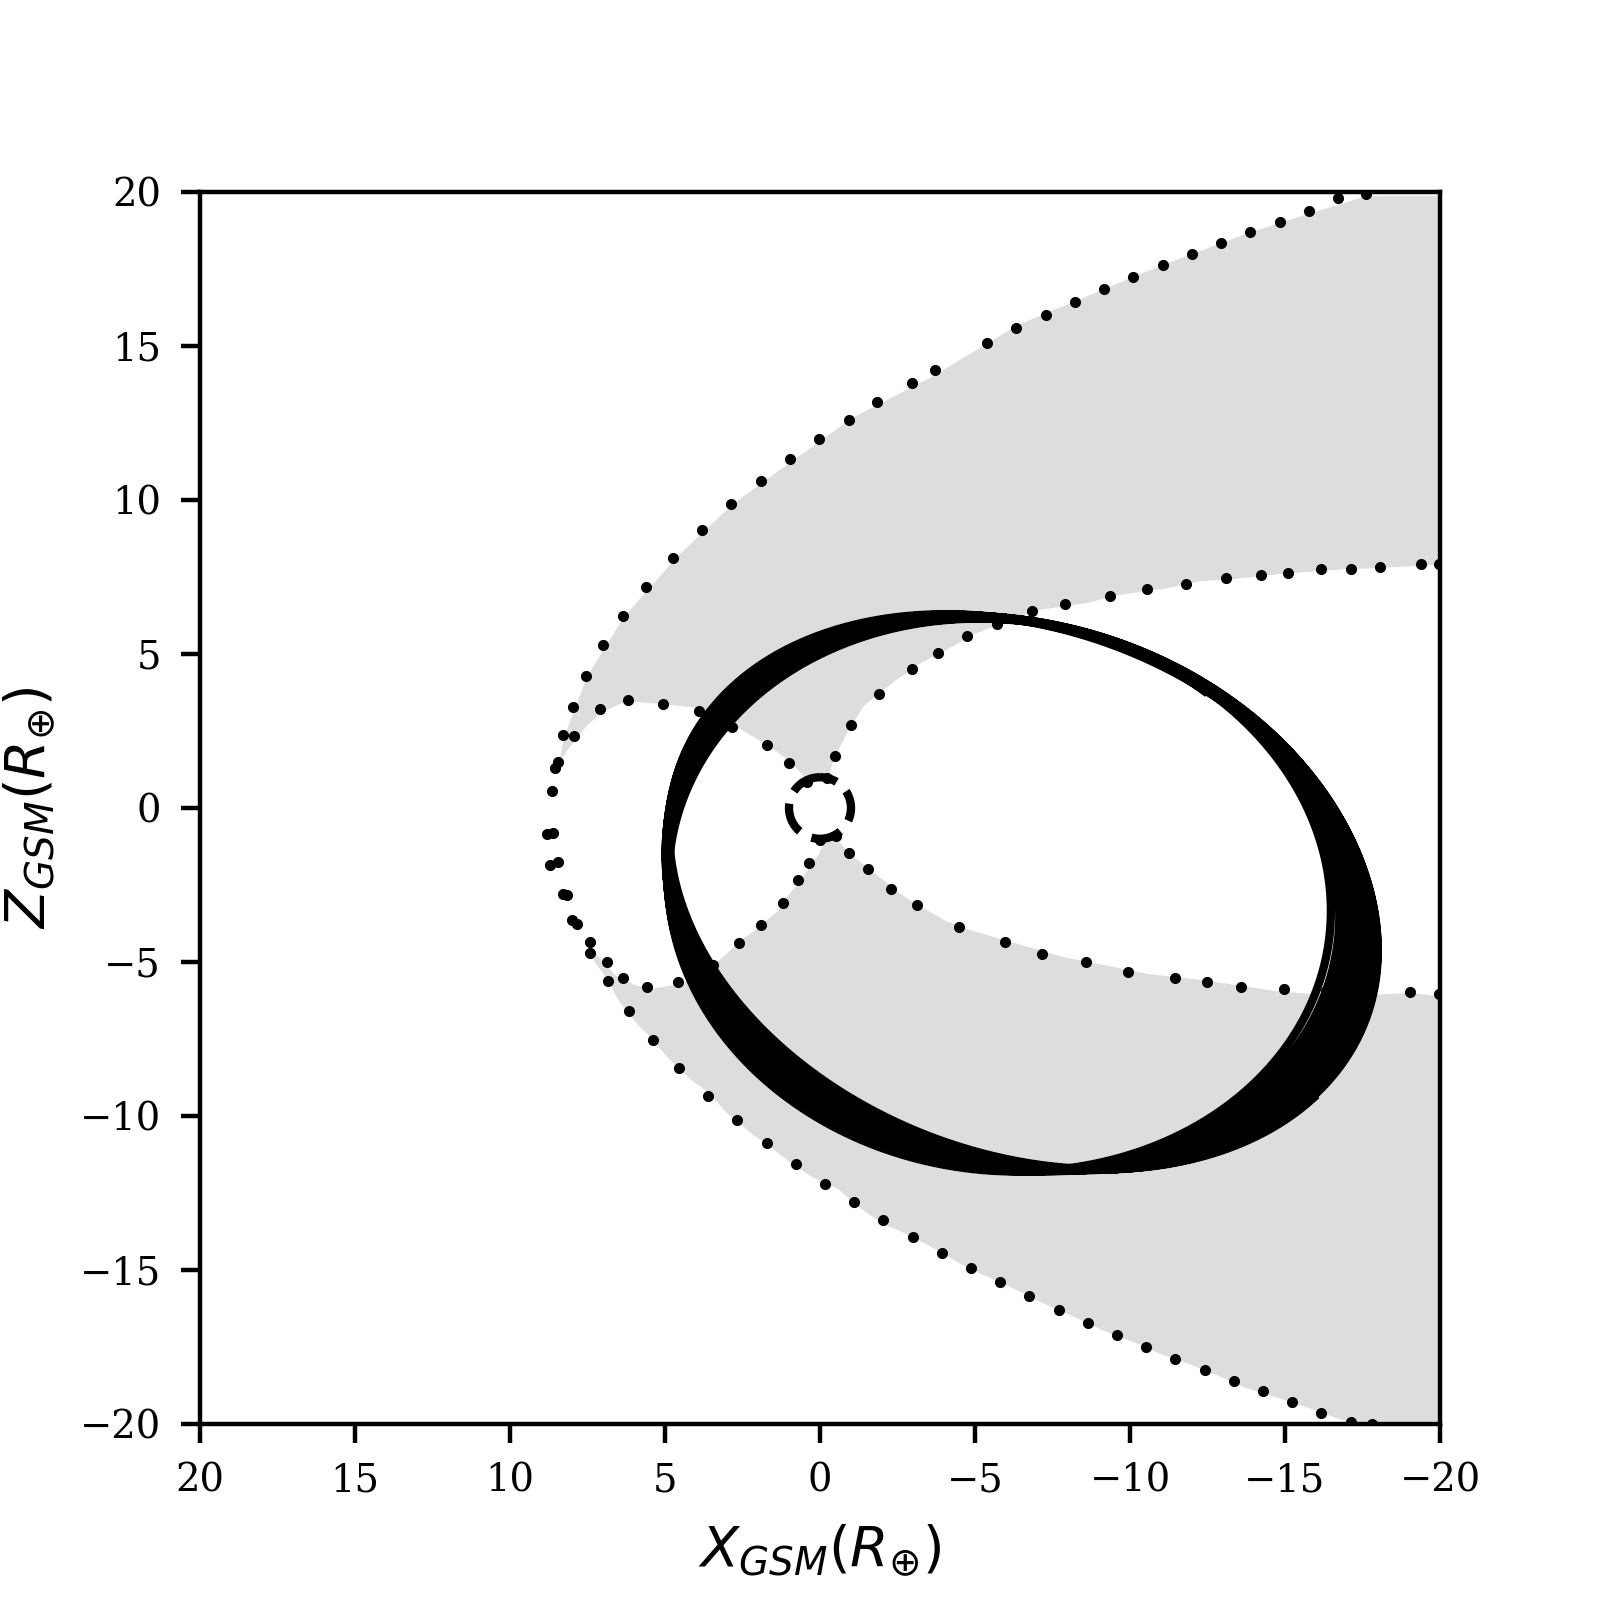
\includegraphics[width=\textwidth]{sc_pos_09_05_coloured.png}
    \end{minipage}\hfill
    \begin{minipage}[c]{0.57\textwidth}
        \captionof{figure}{Plot of Cluster's orbit throughout September 2005 (solid), along with model results for the magnetopause and open-closed boundary on 15/09/2005 (dotted) \cite{Fear1506, substormConfModel}. The grey shaded region is of interest as it contains open field lines. If a reconnection event was detected while the spacecraft was in this region then it could indicate a transpolar arc. Plotting is done in the GSM coordinate system, where +X points to the sun and +Z points along the magnetic dipole axis.}
        \label{fig:ClusterPos}
    \end{minipage}
\end{Figure}

\subsection{High temperatures in the lobe}
Occasionally when Cluster is in the lobe, it will detect periods of uncharacteristically high temperature. There is some debate on the cause of this; Shi \textit{et al} \cite{Shi2013} attribute it to solar wind penetrating into the lobe, whereas Fear \textit{et al} \cite{Fear1506} suggests that this cannot be the case due to the presence of a double loss cone. 

A double loss cone occurs when there is a magnetic mirror at both ends of the field line. This would imply that the observed field line is closed, since the Earth's dipole field has the property where magnetic field strength increases as you travel along a field line to either pole. This would cause an ion to slow down and reverse direction at the poles, i.e. it bounces back and forth from pole to pole.



\subsection{Temperature distribution in the magnetosphere}
Figure \ref{fig:tempLocations} shows the mean distribution of temperatures in the magnetosphere, during the period May to December for years 2002, 2010. We can see the general shape of the plasma sheet, a hot region to the right of the Earth where the normal aurora- generating reconnection happens.

\begin{Figure}
    \begin{minipage}[c]{0.57\textwidth}
        \centering
        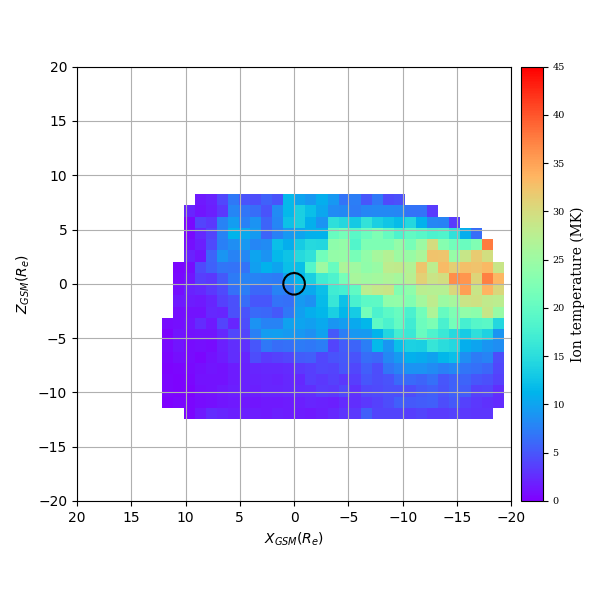
\includegraphics[width=0.9\textwidth]{tempLocations.png}
    \end{minipage}\hfill
    \begin{minipage}[c]{0.4\textwidth}
        \captionof{figure}{Temperature distribution in the magnetosphere. Measurements from Cluster orbits in the months May-December during the years 2002-2010. Each pixel is $1{R_e}^2$ in area, and represents the mean ion temperature when cluster was in that position, blue for lower temperatures and red for hotter. The plasma sheet is visible as a high temperature region to the right of Earth.}
        \label{fig:tempLocations}
    \end{minipage}
\end{Figure}

\subsection{High temperature events}
What constitutes a high temperature? That depends on where in the magnetosphere you are looking. The most easily quantifiable way to separate the plasma sheet from the lobe is to look at the Z coordinate in the Geocentric Solar Magnetospheric (GSM) coordinate system \cite{maus_2006}.

\begin{Figure}
    \begin{minipage}[c]{0.57\textwidth}
        \centering
        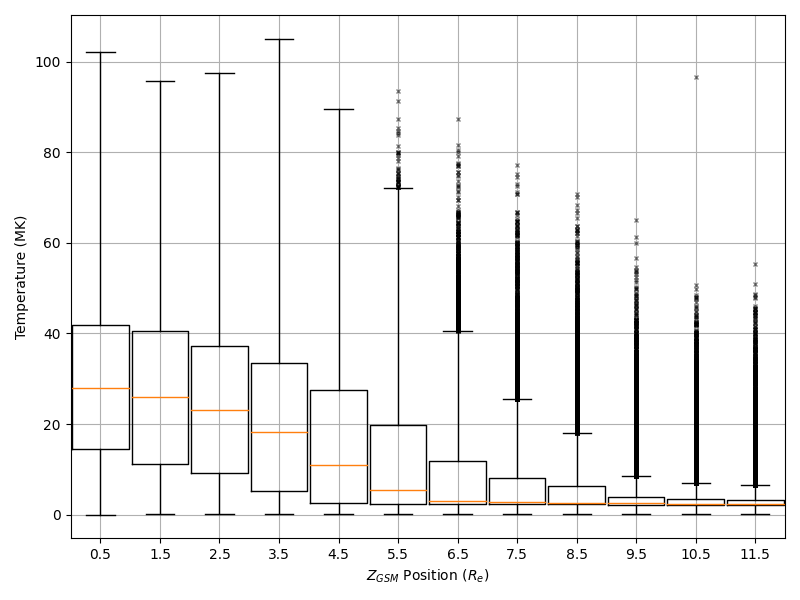
\includegraphics[width=\textwidth]{avg_temp_z.png}
    \end{minipage}\hfill
    \begin{minipage}[c]{0.4\textwidth}
        \captionof{figure}{Box plot of the temperature distribution as a function of $Z_{GSM}$. Each box covers a width of $1R_e$, starting at $[0,1)$ $R_e$ then $[1,2)$ $R_e$ etc until $[11,12]$ $R_e$. Yellow lines represent the median, each box is the interquartile range of each bin, and the ``whiskers'' are maximum and minimum values, up to $3\times IQR$. Outliers are plotted as black `$\times$'. The box centred at $5.5R_e$ (for the interval $[5,6)$ $R_e$) suggests that temperatures above $\approx20MK$ are good candidates for high temperature events. Data is from Jul-Oct 2002-2010 for $X_{GSM}<0$ $R_e$.}
        \label{fig:avg_temp_z}
    \end{minipage}
\end{Figure}

We can see from Figure \ref{fig:tempLocations} that the plasma sheet ends at approximately $Z_{GSM}=\pm6R_e$. Giving an exact position for the edge of the plasma sheet is difficult as it is dynamic and in this project we use measurements from many months and years.

In figure \ref{fig:avg_temp_z} we created a box plot of measurements from July-October 2002-2010 (for $X_{GSM} < 0$, i.e. excluding points sunwards of Earth). Taking the estimation from above that the plasma sheet ends at $\approx6R_e$, we can see from the box centred on $5.5R_e$ that temperatures exceeding $\approx 20MK$ can reasonably be considered uncharacteristically high.

\subsection{Duration of events \label{ssec:DURn}}
The event analysed by Fear \textit{et al} \cite{Fear1506} on 15-09-2005 lasted for approximately 2 hours. In figure \ref{fig:aur_comp} we analyse the length of each of our events detected in the same time period as above (Jul-Oct 2002-2010), plotting the result as a histogram. Repeating this for various cutoff points based on $|Z_{GSM}|$ gives a view of how the length of each event changes over time. 

\begin{Figure}
    \centering
    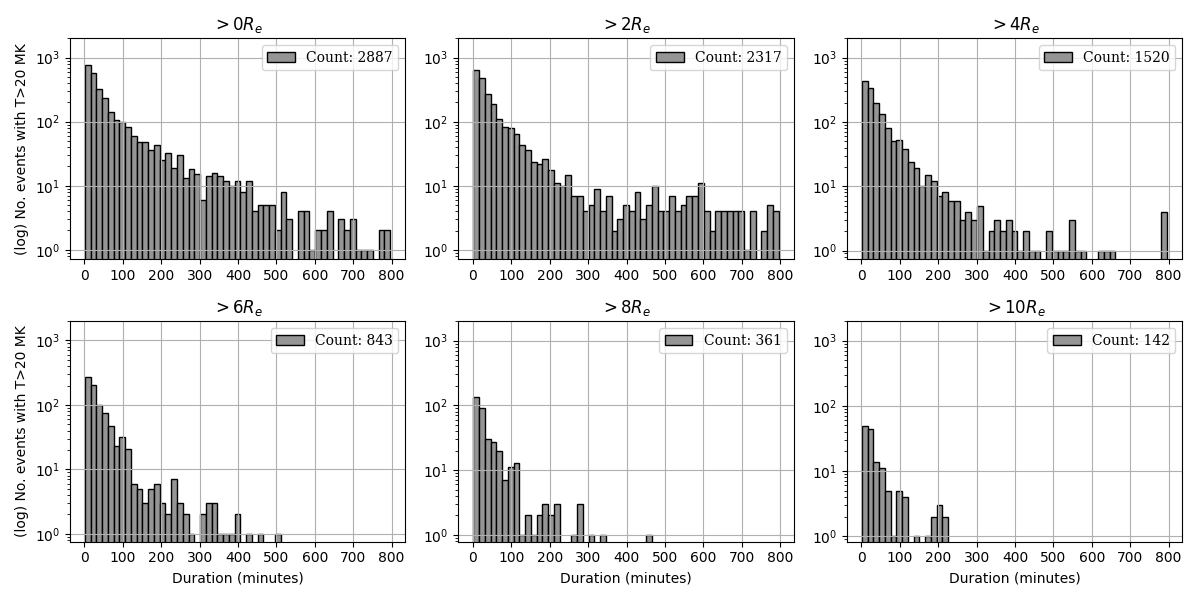
\includegraphics[width=\textwidth]{aur_comp.png}
    \captionof{figure}{Histograms showing the number of events with a certain duration (in minutes). Each panel shows a different cutoff point for $|Z_{GSM}|$. Very long duration events are consistent with passing through the plasma sheet where having a temperature above $20MK$ for over 10 hours is possible. Therefore as the $Z$ cutoff is increased we would expect those long duration events to become less common as measurements outside of the plasma sheet are excluded.}
    \label{fig:aur_comp}
\end{Figure}

We see that when the plasma sheet is excluded by only taking the measurements where $|Z_{GSM}|<6R_e$, there are $732$ events left. This works out to be just under one per day ($732/984\approx0.75\ events/day$). The properties of this distribution are shown in table \ref{tab:event_durn}. This shows that these events are comparable in length to the 15-09-2005 event.

Many short duration events are likely to be noise. Although cluster makes a full rotation approximately every three seconds and can therefore provide measurements with similar resolution, the choice was made to average the data into five minute bins, which would match with the predicted geometric position data from \cite{cdms}, and the IMF components parameters obtained from NASA/GSFC's OMNI data set through OMNIWeb \cite{omniData}. Downsampling the data was chosen over upsampling because using the mean of many measurements is preferable to interpolating missing data. Doing this allows every point to have an associated $x,\ y,\ z,\ B_x,\ B_y,\ B_z\ \& T$

\begin{table}[]
    \begin{minipage}[c]{0.57\textwidth}
        \centering
        \begin{tabular}{||c|l||c|l||}
            \hline
            count & 732 & $25\%$ & 00:15:00 \\
            mean & 01:16:18 & $50\%$ & 00:25:00 \\
            std & 03:38:36 & $75\%$ & 01:00:00 \\
            min & 00:10:00 & max & 1 day 12:40:00 \\
            \hline
        \end{tabular}
    \end{minipage}\hfill
    \begin{minipage}[c]{0.4\textwidth}
        \caption{Statistical properties for the duration of events occurring at $|Z_{GSM}|>6R_e$.}
        \label{tab:event_durn}
    \end{minipage}
\end{table}

\subsection{Interplanetary Magnetic Field \label{interMF}}
The IMF data consists of three measurements from OMNI, $B_x, B_y, B_z$, all in the GSM coordinate system.

$B_z$ represents the IMF polarity, positive northwards and negative southwards. For the time range that we have been considering, the average $B_z$ was:

\begin{equation}
    \overline{B_z} = 0.004 \pm 3.275\ nT
\end{equation}

Therefore it was effectively 50\% positive and 50\% negative. 

\section{Effect of IMF direction on temperature distribution}
Figure \ref{fig:imfDiff} shows the difference between the average temperature distribution (figure \ref{fig:tempLocations}) and an equivalent average when IMF is only northwards. Redder represents an increase in average temperature when IMF is northwards and blue is a decrease.

The interplanetary magnetic field is highly variable which has caused problems with high standard deviation throughout this project, for figure \ref{fig:imfDiff} this has resulted in a lot of noise. However, some notable features are visible. The plasma sheet is cooler during times of northward IMF, this is consistent with previous studies \cite{TAYLOR20081619} saying that the plasma sheet becomes colder and denser during extended times of northward IMF, known as the cold dense plasma sheet (CDPS).

It is also theorised that the plasma sheet expands vertically during northward IMF \cite{huang, nishida}, which could explain the increase in temperature outside of the plasma sheet.

\begin{Figure}
    \begin{minipage}[c]{0.57\textwidth}
        \centering
        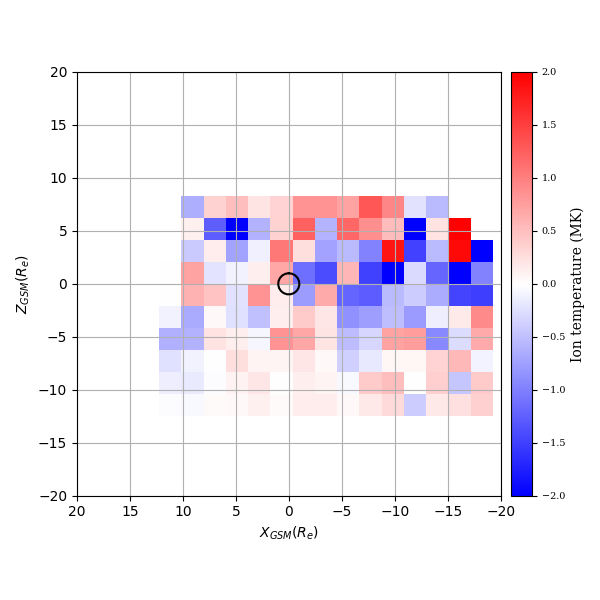
\includegraphics[width=\textwidth]{tempLocations_IMFdiff.png}
    \end{minipage}
    \begin{minipage}[c]{0.4\textwidth}
        \captionof{figure}{Difference plot of average temperature distribution (figure \ref{fig:tempLocations} compared to distribution when IMF is northward. Red indicates a higher average temperature during northward IMF and blue indicated colder. The IMF is highly variable, resulting in a lot of noise, however a decrease in temperature inside the plasma sheet and an increase above and below are still visible. This confirms other direct measurements of the plasma sheet boundary expanding vertically \cite{huang, nishida} and of the cold-dense plasma sheet formation during northward IMF. }
        \label{fig:imfDiff}
    \end{minipage}
\end{Figure}

\section{RESULTS \label{sec:results}}

\subsection{Relationship between $|Z|$ and $B_Z$ for 2005}
If high temperatures in the lobe are caused by times of northward IMF, then we should see that the average IMF $B_Z$ increases with $Z$. 

Initially, we considered only the times between July-October 2005 because we knew for certain there was at least one event during that period, on 15/09/2005 \cite{Fear1506}.

\begin{Figure}
    \begin{minipage}[c]{0.57\textwidth}
        \centering
        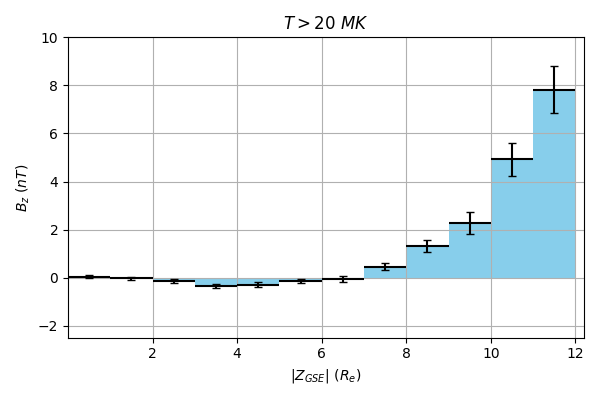
\includegraphics[width=\textwidth]{littleDates_imf_with_z.png}
    \end{minipage}
    \begin{minipage}[c]{0.4\textwidth}
        \captionof{figure}{Bar chart showing the variation of $B_Z$ with $|Z_{GSE}|$. Each bar is the mean IMF value for the $|Z_{GSM}|$ bin [z, $|Z_{GSM}|_{MAX}$]. The height of the bars at $>7R_e$ strongly indicates that high temperatures in the lobe are correlated with northward IMF. However, as shown later - this may not be the case in reality. }
        \label{fig:littleDates_imf_with_z}
    \end{minipage}
\end{Figure}

Figure \ref{fig:littleDates_imf_with_z} shows how the average IMF $B_z$ varies with $Z_{GSE}$. Each bin on the plot contains points from the maximum value on the horizontal axis ($12R_e$) down to the minimum $Z$ of each bin. E.g. the bin beginning at $6R_e$ contains values from $6R_e$ all the way to $12R_e$.

For $|Z_{GSE}|<7R_e$ the average IMF is approximately stationary, which is as expected and aligns with the statement in section \ref{interMF} that IMF $B_Z$ is 50\% positive and 50\% negative on longer timescales. For $|Z_{GSE}|\ge7R_e$ we see a steadily increasing positive trend for the IMF. This would be an indication that high temperatures in the lobe are correlated with northward IMF. 

A correlation with northward IMF suggests that high temperatures in the lobe do not occur during the typical Dungey cycle. If tail reconnection is still happening but dayside reconnection has been halted then there could be a build up of flux in the tail that has nowhere to go apart from spreading into the lobes and becoming trapped. This mechanism was proposed by Milan \textbf{et al} \cite{TPAdebate}, they provide further evidence that this is the cause by showing for the case study on 15/09/2005 that atypically hot plasma occurs on closed field lines.

\subsubsection{Angle of IMF in Y-Z plane}
We further explore this relationship by considering the angle that IMF creates in the GSE Y-Z plane (see diagram on the right below).

Figure \ref{fig:littleDates_imf_angle_hist} shows nine polar histograms, each one containing data points greater than a minimum $|Z|$ threshold (noted above each plot). The bars are normalised so that the area is equal to 1. Each plot also contains a red line, the angle represents the directional mean angle \cite{mardia_jupp_2000} and the length represents the resultant length. 

Each measurement of the IMF can be considered as a vector with an $x$, $y$ and $z$ coordinate, therefore the angle in the $yz$ plane $\theta_{yz}$ can be defined as:

\begin{equation}
    \theta_{yz}= 
    \begin{cases}
        \tan^{-1}\left(\frac{B_y}{B_z}\right) &\text{ if } x>0, \\
        \tan^{-1}\left(\frac{B_y}{B_z}\right)+\pi &\text{ if } x < 0 \text{ and } y \ge 0, \\
        \tan^{-1}\left(\frac{B_y}{B_z}\right)-\pi &\text{ if } x < \text{ and } y < 0, \\
        +\frac{\pi}{2} &\text{ if } x=0 \text{ and } y > 0, \\
        -\frac{\pi}{2} &\text{ if } x=0 \text{ and } y<0, \\
        \text{undefined} &\text{ if } x=y=0
    \end{cases}
\end{equation}

This precise definition, provided by the \verb|arctan2()| \cite{arctan2} function in the 3rd party python package numpy \cite{numpy}, allows for an unambiguous conversion from Cartesian to polar coordinates. 

The mean direction can also be considered the direction of centre of mass, which has coordinates:

\begin{equation}
    \overline{C} = \frac{1}{n}\sum_{j=1}^n \cos\theta_{yz}, \qquad \overline{S}=\frac{1}{n}\sum_{j=1}^n\sin\theta_{yz}
\end{equation}

From which the directional mean can be obtained with \verb|arctan2(|$\overline{S}/\overline{C}$\verb|)|. The resultant length is then simply $R=\sqrt{\overline{S}^2+\overline{C}^2}$.

\begin{Figure}
    \centering
    \incfig[0.3]{angleExample}
    \hspace{2cm}
    \incfig[0.3]{angleReference}
\end{Figure}

Using a directional mean when working with angles is more precise as it allows accurate averaging of a set of vectors spread across the $360^\circ\rightarrow0^\circ$ boundary. For example, imagine a set of angles $[300, 345, 355, 7, 22, 40]$; the numerical mean of these values is $178^\circ$ which, as is clear in the diagram to the right, is almost $180^\circ$ from the true mean and not actually representative of the values at all. The directional mean however comes out to be $359^\circ$, this fits the data much better.

Now back to figure \ref{fig:littleDates_imf_angle_hist}. The bars in each plot show how the distribution varies over the range of $|Z|$, and even without the mean line to guide you it is clear that as $|Z|$ increases the angles are trending towards the upper half, which is $+\text{ve}\ B_z$ i.e. northwards IMF.

Because of the nature of how the directional mean was calculated, each point is treated as a unit vector. This allows a slightly different perspective on the IMF trend to figure \ref{fig:littleDates_imf_with_z}, since it removes bias introduced by the magnitude of $B$. In this case though we see the same trend, starting off negative/almost zero (small resultant length) and trending strongly positive.

\begin{Figure}
    \centering
    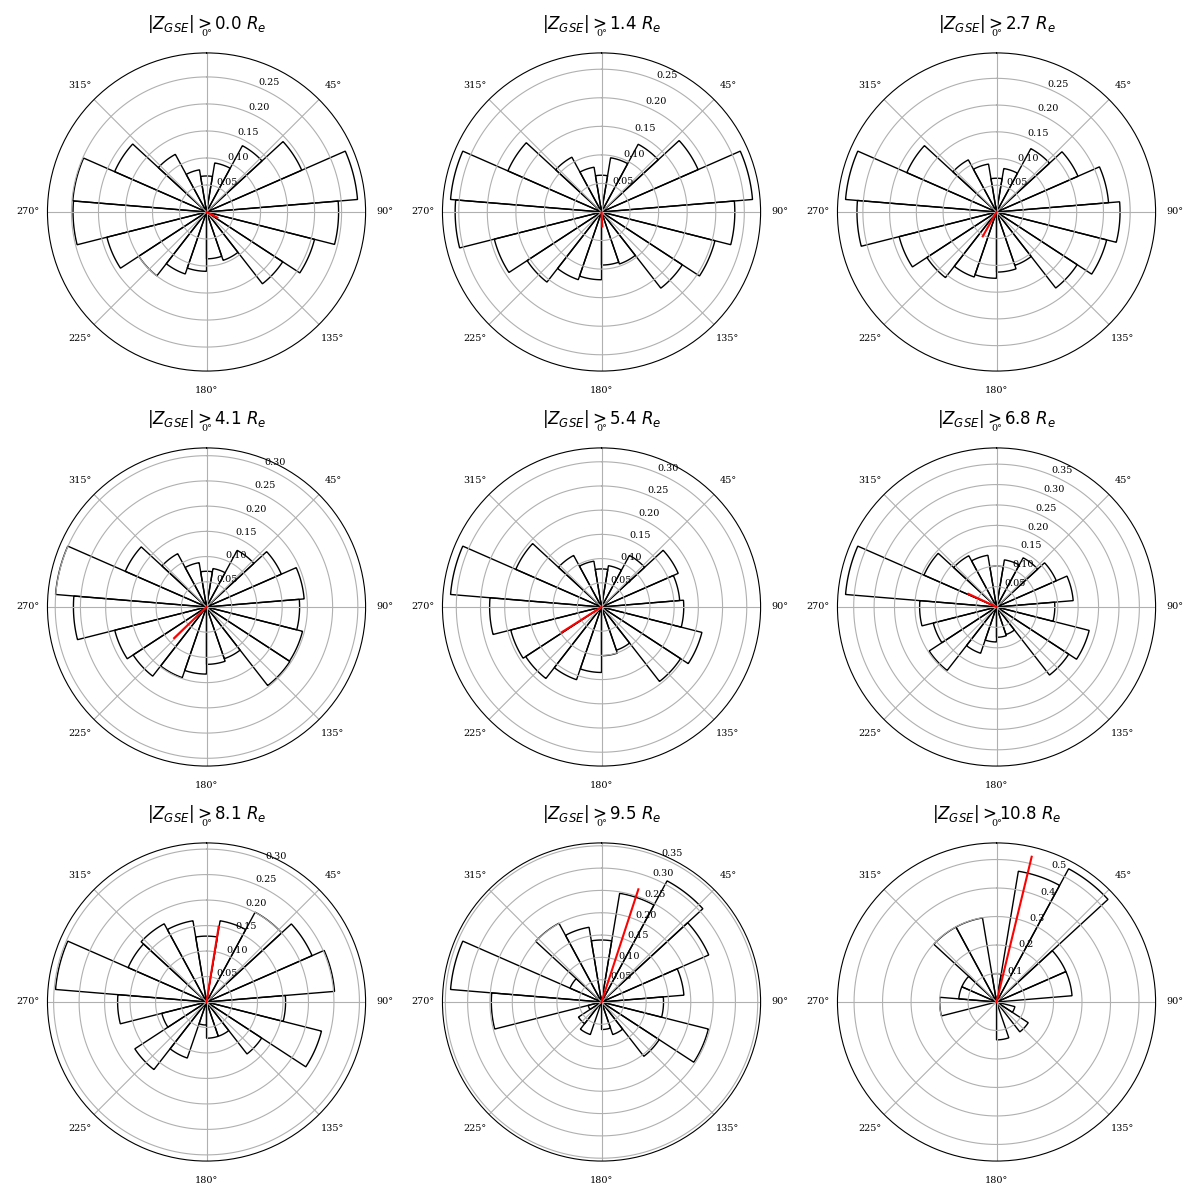
\includegraphics[width=\textwidth]{littleDates_imf_angle_hist.png}
    \captionof{figure}{Polar histograms of IMF $\theta_{yz}$ angle distribution. Bars represent number of events with a particular angle, normalised so the total area equals 1. There are 20 bars per plot each covering an angle of $2\pi/20=0.31$ radians or $17.7$ degrees. Each plot represents a different minimum cutoff value, increasing left-right and top-bottom. The red line on each plot represents the directional mean angle and resultant length of the data in the plot. A short line represents a weak correlation with the mean and a long line represents a strong correlation, i.e. the data all points in roughly the same direction. We see that as $|Z_{GSE}|$ increases, the mean direction line begins to point more northwards and becomes longer.}
    \label{fig:littleDates_imf_angle_hist}
\end{Figure}

\subsection{Expanding to include years 2002-2010}
With the results from July-October 2005 looking so promising, expanding the results to include the full range (2002-2010) was a natural next step. Figure \ref{fig:imf_with_z} shows how this has affected the results. The shape is very similar however the effect is much less pronounced. Figure \ref{fig:littleDates_imf_with_z} shows an increase from $0\ nT$ all the way to a maximum average of $8\ nT$. Here, the increase is less than $1nT$. It appears as though there is still a connection between northward IMF and Z, however the fact that adding more data has caused the mean values to suddenly jump much closer to 0, well below the standard error bars of fig.\ref{fig:littleDates_imf_with_z} at high Z does make the result suspect.

\begin{Figure}
    \begin{minipage}[c]{0.57\textwidth}
        \centering
        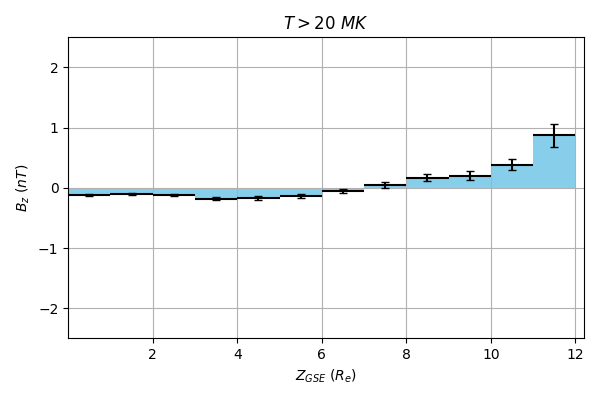
\includegraphics[width=0.9\textwidth]{imf_with_z.png}
    \end{minipage}
    \begin{minipage}[c]{0.4\textwidth}
        \captionof{figure}{Similarly to fig \ref{fig:littleDates_imf_with_z}, plot shows average $B_z$ as a function of $Z$. In this figure, measurements from the whole available range have been considered, that's the months July to October of the years 2002 to 2010. In this plot we see a much more compressed version of the previous, calling into question the results from July-October 2005.} 
        \label{fig:imf_with_z}
    \end{minipage}
\end{Figure}

Since the result from using all months is so different to when 2005 was isolated, it is interesting to compare all the months 2002-2010 side-by-side to see what each year's data looks like. If there were a definite connection between we would expect all years to exhibit the same trend.

Figure \ref{fig:indiv_months_imf_with_z} shows that this is not the case. Only the years 2002 and 2005 show this strong upwards trend. 2003 does also but to a lesser extent. The years 2006 to 2010 show almost no deviation from zero at all.

An investigation into what makes the years 2002 and 2005 so different would make a very interesting extension to this project. the best place to start would be looking into exactly when the periods of highest $B_Z$ occurred during those months.

\begin{Figure}
    \centering
    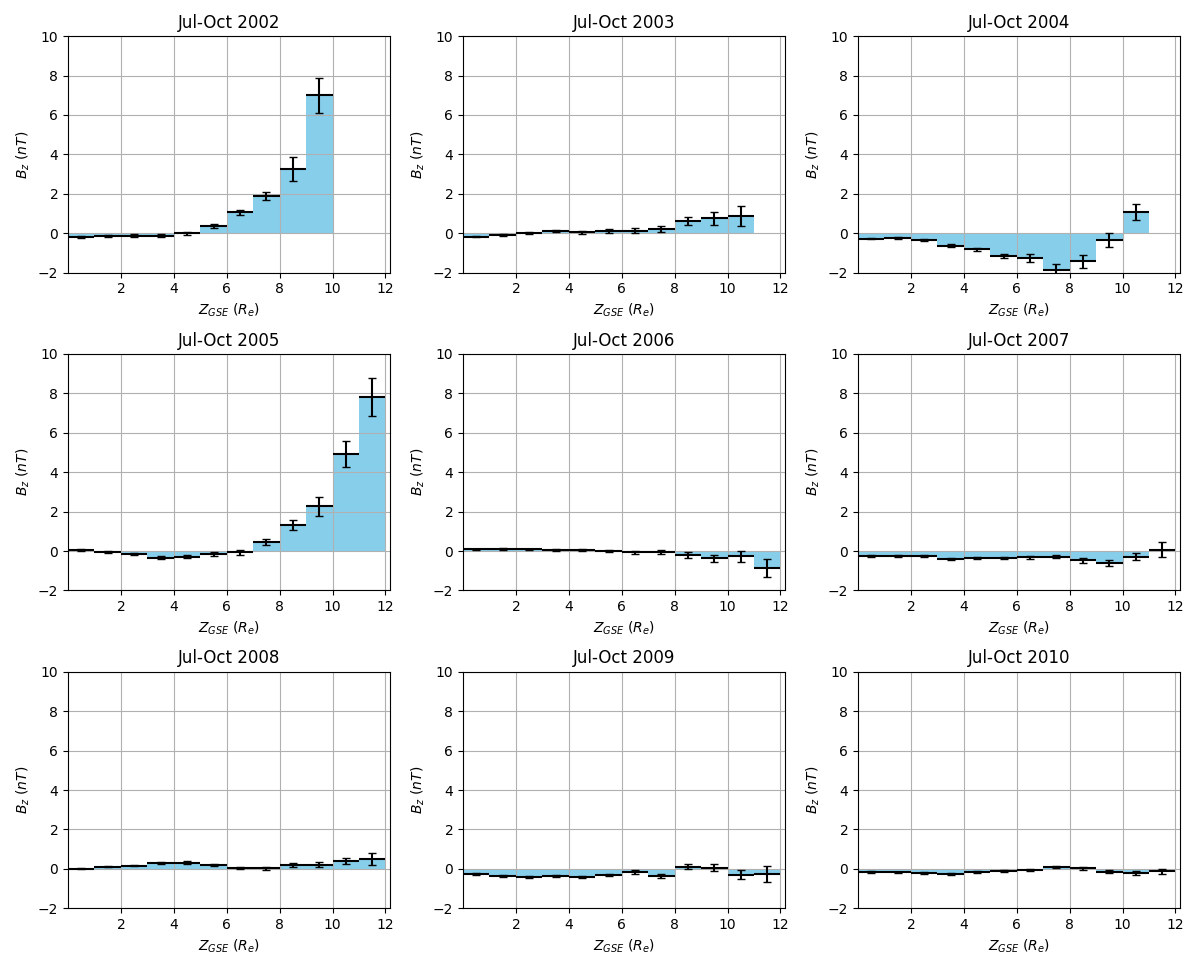
\includegraphics[width=\textwidth]{indiv_months_imf_with_z.png}
    \captionof{figure}{Comparison of years 2002-2010, showing the amount of variability. Only the years 2002 and 2005 show the predicted trend.}
    \label{fig:indiv_months_imf_with_z}
\end{Figure}

Taking a look at figure \ref{fig:imf_angle_hist} where the magnitude of $B$ does not affect the result, we see that the mean angle stays southward for all ranges of $Z$, with the exception of $|Z|>10.8$ where the angle is $53^\circ$, but the resultant length is so short that it's essentially zero. This is further evidence that the relationship is more complex than previously thought.

\begin{Figure}
    \centering
    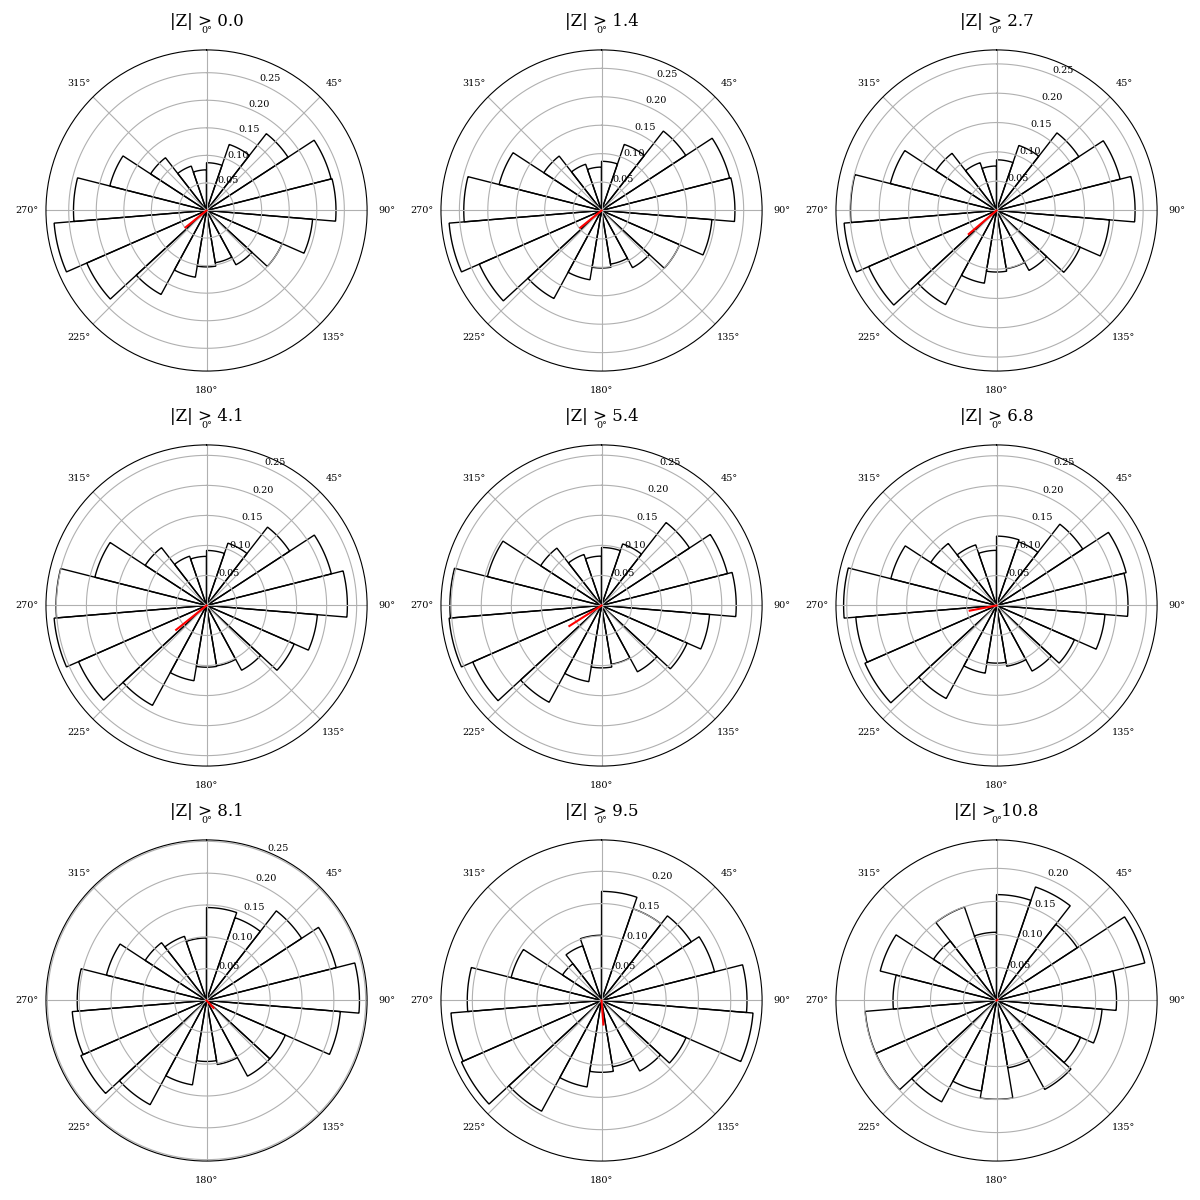
\includegraphics[width=\textwidth]{imf_angle_hist.png}
    \captionof{figure}{Similar to \ref{fig:littleDates_imf_angle_hist}, but including the entire range of years 2002-2010. We see that in this case the average IMF is always negative, except for the last case at $>10.8\ R_e$ where it is zero. This shows that it is certainly not valid to conclude that high temperatures in the lobe are directly correlated with northward IMF.}
    \label{fig:imf_angle_hist}
\end{Figure}

\subsection{Connection to Transpolar Arcs}
It is possible to compare temperatures in the lobe with images of the auroral oval. As shown in section \ref{ssec:DURn}, there were 732 observed events with a temperature of over $20MK$. These can be filtered further to exclude all events with a duration less than 1.5 hours. 

This is to align with observations from SSUSI, an instrument carried on Defence Meteorological Satellite Program (DMSP) satellites that have been taking images of the auroral oval every 100 minutes since 2005. 

Computing power and internet bandwidth were limited during this project, so a full an exhaustive search of all SSUSI instrument data was not possible. Instead, we chose to limit to the F16 dataset only.

Finding a way to classify transpolar arcs automatically proved to also be beyond the scope of this project, though it would be a very interesting future extension. There is simply too much going on in the auroral oval to create an unsupervised machine learning model that distinguishes between an image of the oval that has a TPA and one that does not. A supervised model would be more useful in this instance, however a requirement for supervised learning is to have a labelled dataset to train/test on. This presents two problems:

The first is scarcity of data, there is a maximum of approximately $27,000$ images available from F16 orbits from 2005-2010 assuming F16 completes 15 orbits per day. Transpolar arcs are relatively rare, when labelling a small random sample of 100 images we found 12 that contained convincing transpolar arcs. Assuming that estimate is true for the entire sample, this leaves $3240$ images that contain a transpolar arc. Since we are trying to make a binary classification (does/doesn't have a TPA visible) and the training data needs to be balanced so that biases are not introduced, that leaves a training set of $6480$ images. The general ballpark figure for the size of supervised learning training datasets is $100,000-1,000,000$ images.

The second problem is practicality. Since this project is intended to be an analysis of data that has already been captured, it is pointless to label all historical data manually for the purposes of creating a machine learning model, as it is the labelling itself that is the goal. Though it would be useful for classifying data from future orbits.

Therefore, by filtering our high-temperature events to exclude events with a duration $< 1.5$ hours and with a height $\ge\pm7R_e$ we are left with 56 events. This is a manageable number of events to manually investigate. F16 data is organised into per-orbit files approximately 85MB in size. Downloading and analysing a file of that size with the limitations mentioned above is still to much. However, per-day quicklook plots are also available which are typically under 1MB. 

By searching for the date and time of one of the 56 high-temperature events and visually inspecting the quicklook we were able to make a judgement on whether or not there was a transpolar arc during this time.

\begin{Figure}
    \centering
    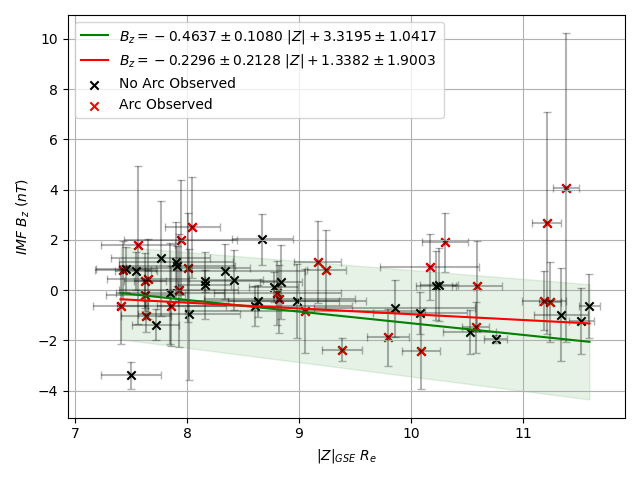
\includegraphics[width=0.7\textwidth]{tpa.png}
    \captionof{figure}{High-temperature events, a black cross shows an event where SSUSI observations did not capture a TPA, red crosses show where a TPA was observed at some point in the duration of the event. The green line is a linear fit to all the data, red line is to just events with a transpolar arc. In both cases, the best fit line is negative. This is significant because it suggests that these events are not linked to northward IMF.}
    \label{fig:tpa}
\end{Figure}

As shown in figure \ref{fig:tpa}, there was a total of 28 events that had an observed arc (exactly 50\%, 15 had IMF $> 0$). It is important to consider that SSUSI instruments do not have a wide enough field of view to capture the entire auroral oval in one pass, and that it is only over the oval for a short period of time. Also, in most cases, dayglow causes the oval at the north pole to be almost entirely obscured. This could potentially explain why there were some high-temperature events without an associated arc.

This sample size is relatively small and could be expanded upon easily by lowering the minimum acceptable length for an event. The current limit of 1.5 hours was chosen so that the F16 satellite has enough time to pass over both poles which should increase the likelihood of a TPA being observed.

However, an arc being visible in 50\% of cases does suggest a link between high-temperatures in the lobe and the formation of transpolar arcs, as it is well above the estimate quoted above of 12\%. 

There were also a large number of transpolar arcs spotted by SSUSI that were not detected by Cluster. This is easily explained by the fact that Cluster is very small and the lobe is very big, it is very likely that Cluster was just in the wrong place to be able to see it.

\section{CONCLUSION}
We looked at data from ESA's Cluster spacecraft mission during the years 2002-2010 to try and determine if there was a link between the polarity of the interplanetary magnetic field and the presence of high temperatures at a distance, $Z$, above or below the Earth.

First, we determined the nominal temperature of the magnetosphere and how it varies with $Z$. As expected, low $Z$ resulted in high temperatures, as the spacecraft would have been in the plasma sheet which is known to be hot. Increasing $Z$ resulted in a decrease in temperature, as the spacecraft moves out of the plasma sheet and into the lobe, a much less active region. The boundary between plasma sheet and lobe changed over time, for the time periods we worked with (July-October 2002-2010) we determined the inner edge of the lobe to be at approximately $\pm6$ Earth radii. Figure \ref{fig:avg_temp_z} showed us that a temperature threshold of above $20MK$ was a good indicator for when the temperature in the lobe was uncharacteristically high.

From here, we expanded to include data from NASA's OMNI spacecraft, which is situated at L1 and provides measurements of many things, including the time-lagged IMF components $B_x$, $B_y$ and $B_z$. Using these, we were able to determine whether the IMF was pointing northward or southward at the time Cluster was taking measurements of the temperature in the lobe. The average $B_z$ was $0.004\pm3.275\ nT$, which confirms the known result that the IMF is 50\% northwards and 50\% southwards.

Using this data, we could then plot the variation in mean $B_Z$ as $|Z|$ increases, but only considering temperatures $T>20MK$. This is because we are interested only in the high-temperature events and because, as shown above - the average $B_Z$ for all $T$ is zero. At first, this analysis was done with a smaller sample of the full dataset, just the months July-October 2005, as it was much faster to work with and we know there was an ideal event discussed in depth by Fear \textit{et al} \cite{Fear1506} that happened during that time, on 15/09/2005. This smaller dataset gave the result that IMF $B_Z$ is strongly correlated with $|Z_{GSE}|$, we confirmed this by looking at the angle the IMF makes on the Y-Z plane, and taking the directional mean along with the resultant length of this angle. This gave a more comprehensive view of the IMF structure and also showed that when the magnitude of $B$ bias was removed, the result stayed the same.

Building upon this, we performed the same analysis on all available data instead of just a sample. With this larger dataset we saw that the initial result did not hold up. Plotting another bar chart showed that the trend has a similar shape, but compressed to over eight times weaker. This meant that instead of the average $B_Z$ increasing to $+8\ nT$ at [11, 12] $R_e$ we only saw an increase of less than $1\ nT$. 

Looking at each year's worth of data individually showed that 2005 was an anomalous year, with 2002 showing a similar trend but all other years showing either a decrease in $B_Z$ or a flat zero, the reasons for this are as yet unknown and would be a good extension to the project, as it appears there are some circumstances where northwards IMF is correlated with high temperatures in the lobe, but this relationship is not always true. 

Exploring further, we found that the average IMF angle distribution did not point northwards at all no matter the value of $|Z|$, this further goes to show that the initial trend is not representative of all time.

Lastly, we took the 732 detected high-temperature events and began to look into the relationship they have with transpolar arcs. This is an area that could be expanded upon in future as we were able to show that - using a reduced dataset - transpolar arcs were occurring in 50\% of occasions when high temperatures were spotted in the lobe, compared to a 12\% occurrence in a random sample. However, we have already seen that drawing conclusions from small samples of data can cause misleading results so it is suggested that this avenue is explored further in future projects.

\printbibliography

\begin{appendices}
\section{Derivation of MHD induction equation \label{app:mhd}}
The magnetohydrodynamic induction equation can be derived from these five equations:

\begin{align}
    \text{Ohm's law:} &\quad \textbf{J}=\sigma(\textbf{E}+\textbf{V}\times\textbf{B}) \\
    \text{Ampere's law:} &\quad \nabla\times\textbf{B}=\mu_0\textbf{J} \\
    \text{Faraday's law:} &\quad \frac{\partial\textbf{B}}{\partial t}=-(\nabla\times\textbf{E}) \\
    \text{Maxwell's equation for magnetism:} &\quad \nabla . \textbf{B}=0 \\
    \text{Vector identity:} &\quad \nabla\times(\nabla\times\textbf{B})=\nabla(\nabla . \textbf{B})-\nabla^2\textbf{B}
\end{align}

\noindent Rearrange  Ohm's law then use Faraday's law:
\begin{align}
    \textbf{E} &= \frac{\textbf{J}}{\sigma}-\textbf{V}\times\textbf{B} \\
    \frac{\partial\textbf{B}}{\partial t} &= \nabla\times\left(\textbf{V}\times\textbf{B}-\frac{\textbf{J}}{\sigma}\right) \\
\end{align}

\noindent Rearrange Ampere's law to get:
\begin{equation}
    \textbf{J}=\frac{\nabla\times\textbf{B}}{\mu_0}
\end{equation}

\noindent Therefore:
\begin{equation}
    \frac{\partial\textbf{B}}{\partial t} = \nabla\times(\textbf{V}\times\textbf{B})-\frac{\nabla\times(\nabla\times\textbf{B})}{\mu_0\sigma}
    \label{pre-eq}
\end{equation}

\noindent The vector identity and Maxwell's equation give:
\begin{equation}
    \nabla\times(\nabla\times\textbf{B})=\nabla(\nabla . \textbf{B})-\nabla^2\textbf{B}=-\nabla^2\textbf{B}
\end{equation}

Which simplifies eq.\ref{pre-eq} to:
\begin{equation}
    \frac{\partial\textbf{B}}{\partial t}=\nabla\times(\textbf{V}\times\textbf{B})+\frac{\nabla^2\textbf{B}}{\mu_0\sigma}
\end{equation}

\end{appendices}

% \end{multicols}
\end{document}
